\subsection{Whole blood}\label{sec:whole-blood}

In what follows, we consider a $16\um\times12\um\times16\um$ domain with periodic
boundaries in the $x$ and $z$ directions and with Dirichlet boundary conditions in the
$y$ direction. The fluid velocity is initially zero except at the top boundary, where it
moves at $12\mmpersec$. In the absence of cells, the flow tends toward steady Couette
flow with a shear rate of $\shear=1000\persec$. This serves as our model near-wall region
of a blood vessel.

For whole blood simulations, we return to the 4-point B-spline, $B_3$, as the IB kernel.
Because some RBC configurations generate large forces, the stopping condition of the
previous section limits us to small timesteps. In the interest of reducing simulation
time, we therefore use backward-forward Euler with $\timestep=50\ns$. In tests, we
observe qualitative agreement between this scheme and the two-stage RK scheme. We have
already settled on an RBC discretization in the previous section. We use the same spiral
method to discretize the platelet, but with 900 data and sample sites. Using the same
number of sample sites and data sites aligns more closely with traditional IB methods. We
also find that the Bauer spiral places points more densely along the edge of the
platelet, which is helpful in resolving the large curvatures there. We parametrize the
surface of the endothelium over $(\theta,\,\varphi)\in[0,\,2\pi)^2$ with reference shape
\begin{equation}
    \vec{\hat{X}}_\text{endo}(\theta,\,\varphi) = \left[\begin{array}{c}
            16\um\cdot(\theta/2\pi)  \\
            y(\theta,\,\varphi) \\
            16\um\cdot(\varphi/2\pi)
    \end{array}\right],
\end{equation}
where $y(\theta,\,\varphi)$ depends on the shape under study. The endothelium is
discretized using 16000 points, defined by the spiral
\begin{align*}
    \varphi_i &= 2\pi (i-1)/N, \\
    \theta_i &= \modulo\left(\left\lceil\!\sqrt{N}\mskip\thinmuskip\right\rceil\varphi_i,\,2\pi\right).
\end{align*}
We consider two shapes for the endothelium. The first, $y=1\um$, emulates the flat wall
typically used in near-wall simulations of RBCs or platelets. The other attempts to
recreate the elongated endothelial cell shape typical of exposure to high-shear
conditions,
\begin{equation*}
    y(\theta,\,\varphi) = 0.75\um + 1\um\cdot\cos^2(\theta-\varphi)\sin^2(\varphi/2).
\end{equation*}
The bumps have a prominence of $1\um$. The endothelial surface is raised by $0.75\um$ to
avoid it interacting with the domain boundary. The positions of the surface are chosen to
maintain a fixed hematocrit of approximately 34\% for both endothelial shapes.

As a preliminary validation of the platelet model and to establish baseline platelet
motion, we consider two platelets along a flat wall. They are placed parallel to the wall
at distances of $0.3\um$ and $0.5\um$. The domain does not contain any RBCs. At a
distance of $0.3\um$, the platelet is expected to ``wobble'', in which the platelet tilts
slightly upward and downward, periodically~\cite{King:2005fv}. On the other hand, the
platelet initially $0.5\um$ from the wall should tumble end-over-end. We observe wobbling
at a frequency of approximately $10\persec$ and tumbling with a frequency of
approximately $30\persec$. These figures are in reasonable agreement with other studies~%
\cite{King:2005fv}. We also note that the edge of the tumbling platelet remains pointed
towards the wall for only 3--$4\ms$.

\subsubsection{Initialization}\label{sec:blood-init}

We assume that the platelets have already been marginated by the RBCs. We think of the
domain as having three layers with the endothelium at the bottom, RBCs on top, and
platelets in between. We begin by settling the endothelium and RBCs before placing
platelets in the space between the RBCs and the endothelium.

In addition to the endothelium, we place 2 rows of 4 RBCs, each in their reference
configuration, in the domain with the RBCs' centers of mass on the plane $y=6\um$.
Because the domain is not wide enough to accommodate two reference RBCs alongside one
another, the cells are staggered by $2\um$. These locations are then randomly translated
and rotated while maintaining a distance of at least $2h$ between cells.

Before placing any platelets in the domain, we allow the flow to develop with only the
endothelium and RBCs. We allow the initialization to continue until at least $17\ms$,
which is approximately when the first RBC overtakes its neighbor. From here, we choose a
series of times, sampled from a Poisson distribution to be approximately $3\ms$ apart, at
which to begin simulations with platelets.

The RBCs for each of the chosen starting configurations are considerably and
unpredictably deformed and have left a space of a few microns above the endothelium
in which we place platelets. To find reasonable starting orientations for the platelets,
we randomly choose points on the endothelium and one on each platelet surface. Each of
the simulations in the upcoming sections contains two platelets, so we choose two points
on the endothelium that are at least $3.9\um$, a platelet diameter plus $4h$, apart. The
resulting platelets are spaced far enough apart to not intersect. We compute normal
vectors on the surfaces of the endothelium and platelets at these points. We orient the
platelets so that the normal emanating from the platelet opposes the normal at the
corresponding point on the endothelium. The platelet is then placed so its chosen surface
point is separated from the endothelium point by a random distance between $0.3\um$ and
$1\um$. If the generated orientation does not pass within $0.4\um$ of an RBC, the
platelet is accepted. Otherwise, we try again with a different platelet point. This
algorithm typically succeeds within 2 attempts.

This initialization process is performed once for each endothelial configuration and we
take the first four acceptable initial configurations for each. In the following section,
we present behaviors found in these simulations. As a point of comparison, we also
consider the same initial configurations for the bumpy wall with the RBCs removed from
the domain.

\subsubsection{Characterization of flow and cell behaviors}

In this section, we catalog the differences in the flow between whole blood along a bumpy
and flat wall, and between flow along a bumpy wall with and without RBCs. We aim to
compare the interactions platelets have with RBCs and the endothelium for these test
cases.
%We begin with the expected behaviors before moving on to remarkable ones.

\begin{figure}[tp!]
    \centering
    \begin{tikzpicture}[spy using outlines={rectangle, magnification=3,connect spies}]
        \begin{axis}[
                axis lines=center,
                xmin=0,
                xmax=12.5,
                ymin=0,
                ymax=12.5,
                ylabel={$y$ ($\um$)},
                xlabel={fluid speed ($\mmpersec$)},
                xlabel near ticks,
                ylabel near ticks,
                legend pos=south east,
                legend style={draw=none}
            ]
            \addplot[color=tol/contrast/red, very thick, x filter/.code={\pgfmathparse{\pgfmathresult*10}\pgfmathresult}] table [x index=1, y index=0] {rpefast1.prof.dat};
            \addlegendentry{\cmark~bumps\hspace{0.5em}\cmark~RBCs};
            \addplot[color=tol/contrast/blue, very thick, x filter/.code={\pgfmathparse{\pgfmathresult*10}\pgfmathresult}] table [x index=1, y index=0] {rpeflat1.prof.dat};
            \addlegendentry{\xmark~bumps\hspace{0.5em}\cmark~RBCs};
            \addplot[color=tol/contrast/yellow, very thick, x filter/.code={\pgfmathparse{\pgfmathresult*10}\pgfmathresult}] table [x index=1, y index=0] {pefast1.prof.dat};
            \addlegendentry{\cmark~bumps\hspace{0.5em}\xmark~RBCs};

            \coordinate (spypoint) at (axis cs: 0.5, 1);
            \coordinate (spyviewer) at (axis cs: 2.5, 10);
            \spy[width=2cm,height=2cm] on (spypoint) in node [fill=white] at (spyviewer);
        \end{axis}
    \end{tikzpicture}
    \caption[A comparison of fluid velocity profiles]{%
Time- and space-averaged fluid velocity profiles for each of the test cases. The
inclusion of RBCs (red and blue curves) causes the region inhabited by platelets,
1--$4\um$, to experience a higher shear rate than it would without RBCs (yellow curve).
    }\label{fig:flow-profiles}
\end{figure}

Flow profiles are shown in Figure~\ref{fig:flow-profiles}. The most notable difference
among the three flow profiles is the nearly Couette flow when RBCs are absent. The only
distinction between this and Couette flow with $\shear=1000\persec$ is the smoother
transition at the wall due to the bumps. This is also the distinguishing feature between
the profiles corresponding to bumpy and flat walls in the presence of RBCs. The smooth
transition from the bumps results in marginally slower flow speeds throughout the domain,
compared to the flat wall. The inclusion of RBCs causes the bends in the red and blue
curves around $y = 3\um$ and $y = 9\um$. Platelets located between $y=1\um$ and $y=3\um$
experience higher shear rates than in simulations featuring RBCs than in those without
RBCs. The region near the upper boundary also experiences an increased shear rate. In
pressure-driven flow through a tube, we expect parabolic flow. The bend near $y = 9\um$
is therefore nonphysical and arises from satisfying boundary conditions at the top
boundary. However, the increased shear rate in the region between $y = 9\um$ and $12\um$
seems to be useful in deterring RBCs from approaching the upper boundary. This region
acts as another RBC-free layer where the RBCs excurse only infrequently. An exclusionary
region of just 1--$2\um$ along the top boundary increases the effective hematocrit to
37--41\%. Furthermore, the reduced shear rate in the region containing RBCs results in
slower tank-treading compared to a dilute suspension of RBCs, with one period now lasting
approximately $40\ms$.

RBCs are effective at preventing the platelets from moving too far from the endothelium.
The furthest observed distance from the endothelium any platelet takes is just under
$1.5\um$. Likewise, RBCs infrequently enter the RBC-free layer, with some notable
exceptions, discussed below. We do not observe any platelet wobbling. Instead, platelets
transiently follow the curve of the bumpy walls, tilt down into the valleys between
bumps, and tumble. Nothing suggests that bumps in the surface of the endothelium alone
can sequester platelets, nor do we directly observe stagnation zones.

\begin{figure}[th!]
    \begin{subfigure}[t]{0.5\textwidth}
        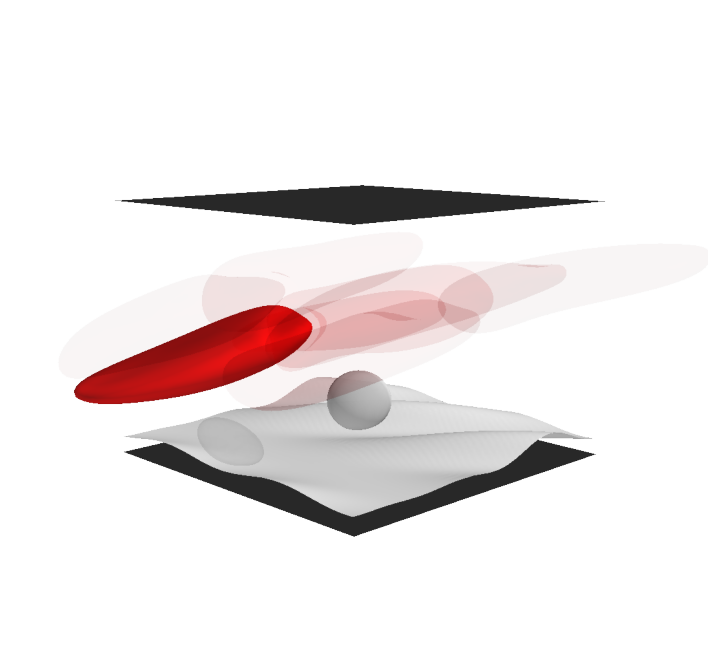
\includegraphics[trim=50 75 50 125, clip, width=\textwidth]{figures/unicycle1.png}
        \subcaption{$t = 46\ms$}
    \end{subfigure}%
    \begin{subfigure}[t]{0.5\textwidth}
        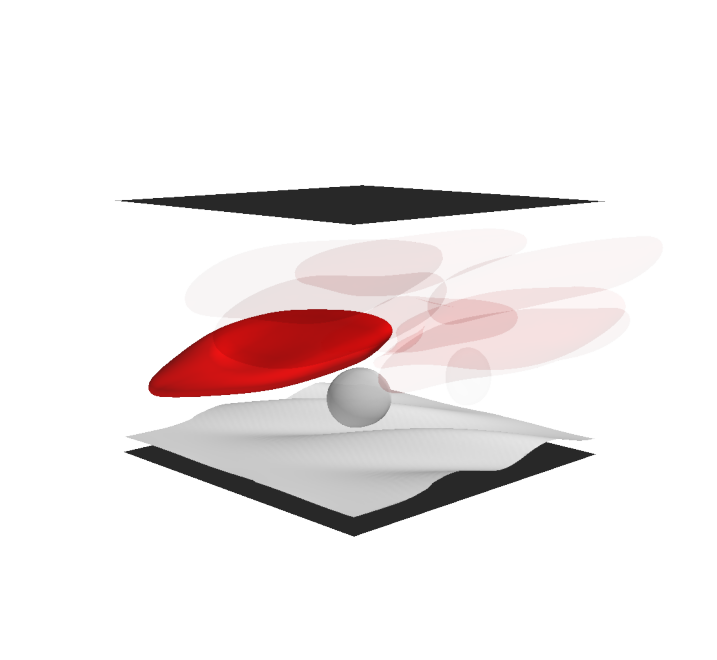
\includegraphics[trim=50 75 50 125, clip, width=\textwidth]{figures/unicycle2.png}
        \subcaption{$t = 48\ms$}
    \end{subfigure}

    \vspace{11pt}

    \begin{subfigure}[t]{0.5\textwidth}
        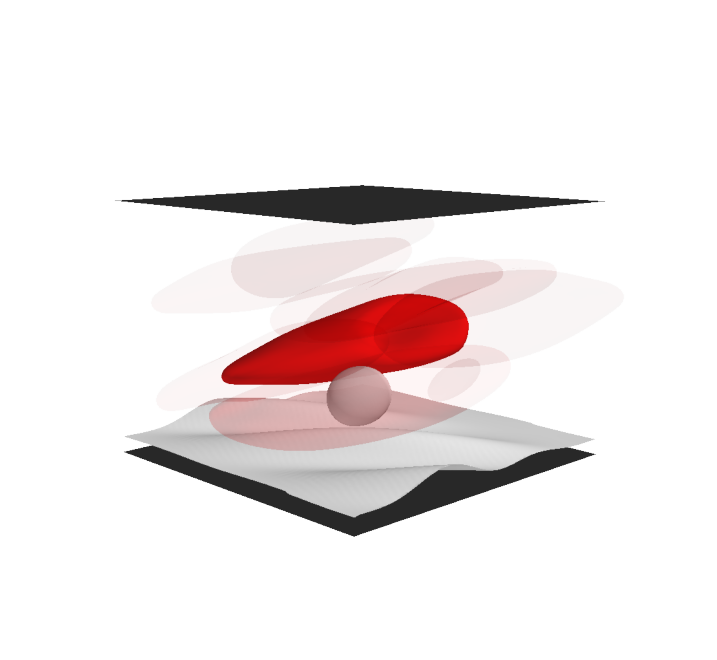
\includegraphics[trim=50 75 50 125, clip, width=\textwidth]{figures/unicycle3.png}%
        \subcaption{$t = 50\ms$}
    \end{subfigure}%
    \begin{subfigure}[t]{0.5\textwidth}
        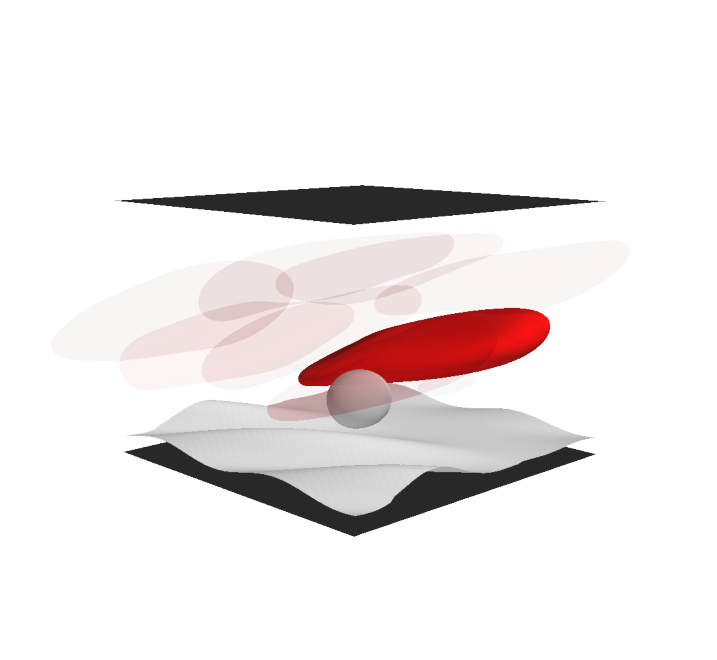
\includegraphics[trim=50 75 50 125, clip, width=\textwidth]{figures/unicycle4.png}%
        \subcaption{$t = 52\ms$}
    \end{subfigure}

    \vspace{11pt}

    \begin{subfigure}[t]{\textwidth}
        \begin{tikzpicture}
            \begin{axis}[
                width=\textwidth,
                height=2in,
                axis lines=center,
                xmin=8.5,
                xmax=61.5,
                ymin=0,
                ymax=0.95,
                ylabel={distance ($\um$)},
                xlabel={time ($\ms$)},
                xlabel near ticks,
                ylabel near ticks
            ]
                \addplot[color=tol/vibrant/magenta, very thick] table [x index=0, y index=6] {rpefast0.dat};
                \addplot[no marks, color=black, dashed] coordinates {(8.5, 0.4)
                                      (61.5, 0.4)};
                \path[name path=axis] (axis cs: 8.5, 0) -- (axis cs: 61.5, 0);
                \addplot[opacity=0, name path=unicycle] table [x index=0, y index=4] {rpefast0.dat};
                \addplot[fill=tol/vibrant/magenta, fill opacity=0.2] fill between[of=unicycle and axis];

                \node at (axis cs: 10.5, 0.9) {(e)};
            \end{axis}
        \end{tikzpicture}
    \end{subfigure}
    \caption[Platelet unicycling behavior]{%
(a)--(d) Snapshots of a platelet rolling on its edge (``unicycling'') with RBCs, one
translucent, flanking either side. The camera tracks the opaque platelet. It's motion is
indicated by the endothelium moving from right to left. (e) The distance between
the platelet and the endothelium. The shaded region indicates that the orientation of the
platelet's short axis is within $45^\circ$ of the vorticity direction.  The black dashed
line indicates $2h$ and is the maximum distance that might be considered contact with the
endothelium. See~\ref{sec:supp} for a video corresponding to this simulation.
    }\label{fig:unicycle}
\end{figure}

Bumpy endothelium simulations without RBCs mimic those with a flat wall; platelets move
away from the wall to a point where they are free to tumble. Unsurprisingly, we observe
platelet tumbling for both flat and bumpy walls with RBCs as well. In Stokes-like flow, a
rigid platelet would tumble faster in flow with a higher shear rate. We might therefore
expect the platelet to tumble faster with RBCs. However, RBCs can significantly disturb
the fluid around a platelet, speeding up its motion, slowing it down, or preventing a
tumble altogether.

We observe platelets rolling in the flow direction along their edge. Because the
platelet in this arrangement is aligned vertically, part of the edge stays in
near-contact with the endothelium while the opposite edge extends into the region
occupied by RBCs.  Contact with RBCs is frequent. These contacts can have a destabilizing
effect, but may also prolong the rolling. Figure~\ref{fig:unicycle}(a)--(d) consists of a
series of snapshots illustrating the behavior. The platelet in this case is flanked by
two RBCs, so it does not have the space to topple over until the RBCs pass a few
milliseconds later.

While Figure~\ref{fig:unicycle} shows this phenomenon on a bumpy wall, it can also occur
above a flat wall. We first observed this motion with a flat wall, and there it lasted
over $40\ms$. The motion was maintained, in part, by an RBC that rode along the top of
the platelet, partially enveloping that platelet. We say that a platelet rolling on its
edge is \term{unicycling}. Figure~\ref{fig:unicycle}(e) illustrates that the platelet
spends more time in contact or near-contact with the endothelium while unicycling
compared to the tumbles near $t=16\ms$ and $t=29\ms$. Though RBCs seem to control the
duration of the unicycling, they are not strictly necessary for unicycling to occur. In
tests with a bumpy wall without RBCs, unicycling is initiated when a platelet rolls
sideways, relative to the flow direction, off of a bump. Without RBCs, the platelet
maintains the vertical alignment for a majority of the simulation thereafter. However,
without frequent interaction with RBCs, the platelet in these simulations move away from
the wall.  Moreover, while we have not observed it directly, we expect that a lone
platelet traveling over a flat wall would also exhibit unicycling, given the right
initial orientation.

\begin{figure}[th!]
    \begin{subfigure}[t]{0.5\textwidth}
        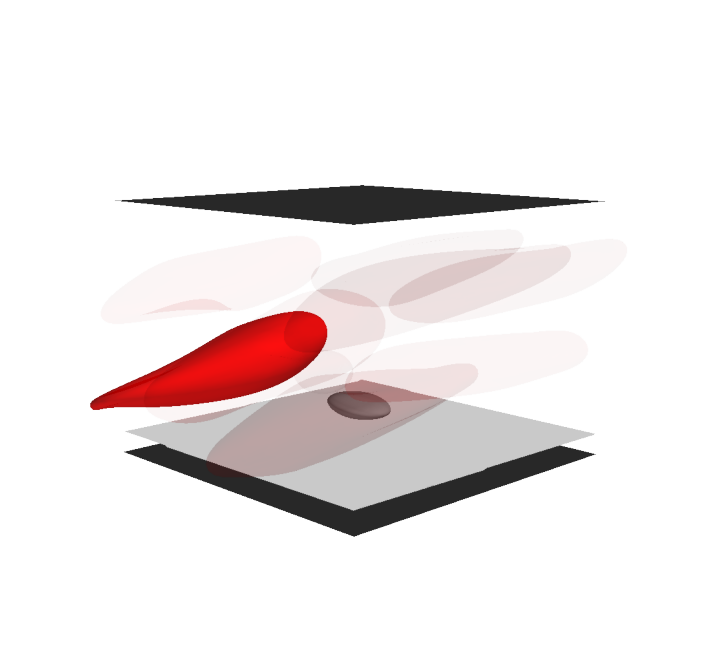
\includegraphics[trim=50 75 50 125, clip, width=\textwidth]{figures/flyover460.png}%
        \subcaption{$t = 46.0\ms$}
    \end{subfigure}%
    \begin{subfigure}[t]{0.5\textwidth}
        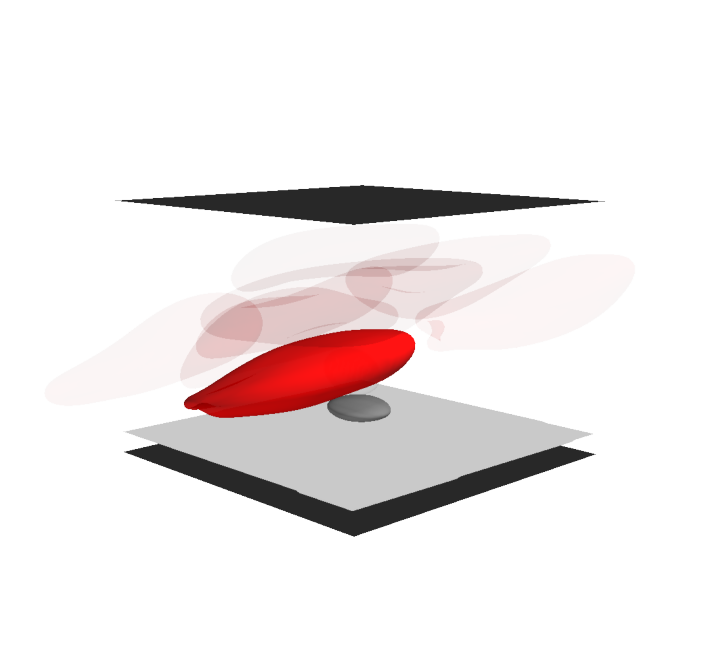
\includegraphics[trim=50 75 50 125, clip, width=\textwidth]{figures/flyover495.png}
        \subcaption{$t = 49.5\ms$}
    \end{subfigure}

    \vspace{11pt}

    \begin{subfigure}[t]{0.5\textwidth}
        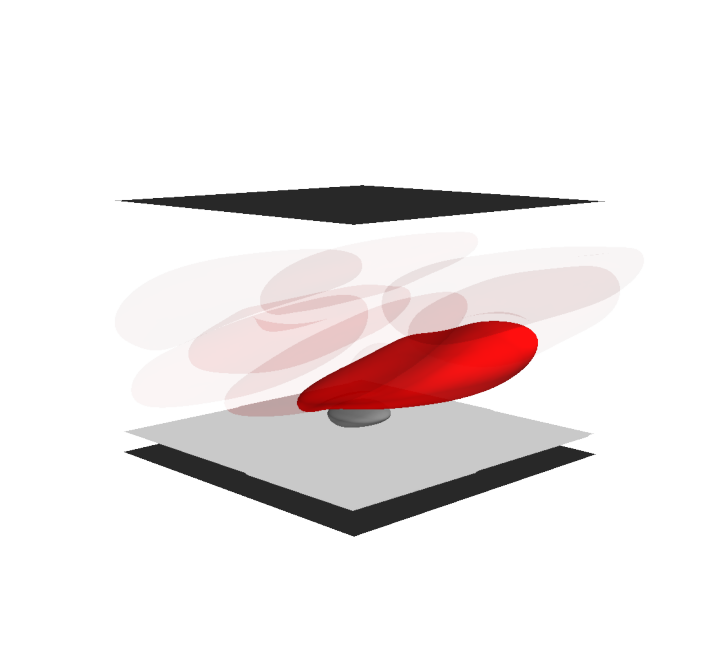
\includegraphics[trim=50 75 50 125, clip, width=\textwidth]{figures/flyover530.png}%
        \subcaption{$t = 53.0\ms$}
    \end{subfigure}%
    \begin{subfigure}[t]{0.5\textwidth}
        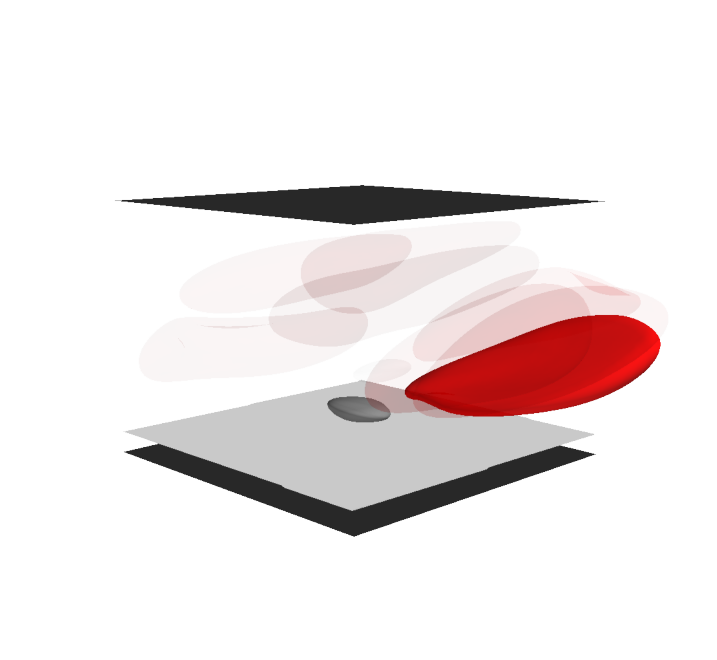
\includegraphics[trim=50 75 50 125, clip, width=\textwidth]{figures/flyover565.png}%
        \subcaption{$t = 56.5\ms$}
    \end{subfigure}

    \vspace{11pt}

    \begin{subfigure}[t]{\textwidth}
        \begin{tikzpicture}
            \begin{axis}[
                width=\textwidth,
                height=2in,
                axis lines=center,
                xmin=8.5,
                xmax=61.5,
                ymin=0,
                ymax=3.25,
                ylabel={velocity ($\mmpersec$)},
                xlabel={time ($\ms$)},
                xlabel near ticks,
                ylabel near ticks
            ]
                \addplot[color=tol/vibrant/magenta, very thick] table [x index=0, y index=3] {rpeflat3.vel.dat};
                \path[name path=axis] (axis cs: 8.5, 0) -- (axis cs: 61.5, 0);
                \addplot[opacity=0, name path=deformed, y filter/.code={\pgfmathparse{#1*3}\pgfmathresult}] table [x index=0, y index=4] {rpeflat3.vel.dat};
                \addplot[fill=tol/vibrant/magenta, fill opacity=0.2] fill between[of=deformed and axis];

                \node at (axis cs: 10.5, 3) {(e)};
            \end{axis}
        \end{tikzpicture}
    \end{subfigure}
    \caption[RBC-mediated platelet-endothelial collision]{%
(a)--(d) Snapshots of RBC-mediated collision between a platelet and the endothelium. (a)
The platelet attempts to tumble. (b)--(c) An RBC comes into proximity with the platelet,
deflects to avoid the platelet, and pushes the platelet into the endothelium, thereby
preventing the platelet from tumbling. (d) The platelet is free to tumble again. (e) The
minimum velocity on the surface of the platelet. The shaded region indicates that the
relative change in aspect ratio of the major axes exceeds 4\%. See~\ref{sec:supp} for a
video corresponding to this simulation.
    }\label{fig:rbc-plt-endo-collision}
\end{figure}

We notice that in simulations with a bumpy endothelium, platelets collide with the bumps.
This tends to occur while the platelet is tumbling, and the edge of the platelet makes
contact with the endothelium. This interaction is characterized by deformations that
flatten the edge of the platelet and a \midtilde5\% relative change in the aspect ratio
of the major axes of the platelet. However, the collision need not occur along the edge
of the platelet, nor, indeed, against a bump in the endothelium. Somewhat surprisingly,
collisions with a flat wall occur at roughly the same frequency, suggesting that RBCs
mediate this behavior. A clear case of this is illustrated in Figure~%
\ref{fig:rbc-plt-endo-collision}(a)--(d). We also note that the few milliseconds
preceding the unicycling in Figure~\ref{fig:unicycle} correspond to a collision with the
wall, showing that this is yet another trigger for unicycling to occur.

Because the platelet comes into contact with the endothelium, or nearly does so, the
platelet slows along the area of contact. Figure~\ref{fig:rbc-plt-endo-collision}(e)
shows the correlation between the relative change in aspect ratio and the reduction in
minimum platelet surface velocity. Though the aspect ratio of the platelet changes
somewhat while normally tumbling, changes of this magnitude seem to always correspond to
interactions with the endothelium. Collisions with the RBC, for example, result primarily
in deformation of the RBC and deflection of the platelet, which is otherwise relatively
unperturbed.
